\chapter{Results for Three-Dimensional Edwards Anderson Model in 
an Externel Field}
\label{chap:sg_result}
This following chapter is a work titled {\bf Parallel Tempering Simulation of 
the three-dimensional Edwards-Anderson Model  with  Compact Asynchronous 
Multispin Coding on GPU}, submitted for publication in Physics Review E.

In this paper, we discussed the results Monte Carlo
Simulation of 3D Edwards-Anderson model.

This paper is written in collaboration with Ye Fang, Ka-Ming Tam, Zhifeng Yun, 
Juana Moreno, J. Ramanujam and Mark Jarrell. 

The idea of the project was first proposed by Ka-Ming Tam. 
Ye Fang and I developed the implementation together. With the code, I ran simulations
on the GPU clusters, accumulated and analyzed all the data. 

This paper is written in collaboration with Ye Fang, Ka-Ming Tam, Juana Moreno, 
and Mark Jarrell. I started a first draft, including the introduction, the 
simulation methods, the measured quantities and the conclusions. I also plotted 
all the figures from the data obtained in the simulation. 
Ka-Ming contributed to the introduction and conclusions. Juana Moreno
and Mark Jarrell also reviewed the paper and improved the conclusions.


\section{Introduction} 
Most spin systems order when the temperature is sufficiently low. 
Conventional magnetic orderings break the spin symmetry, and the moments align 
in a pattern with long range order. However, magnetic 
systems with random frustrated couplings can avoid conventional 
ordering by breaking ergodicity. Typical spin glass systems with 
such competing magnetic couplings include localized spins in metals coupled 
via the oscillating Rudermann-Kittel-Kasuya-Yosida 
exchange as CuFe and CuMn, and in insulators with competing interactions 
as in LiHoYF and EuSrS \cite{Binder-Young-1986,Mydosh-1993,Diep-2004}. These 
systems do not display long range order for a wide range of diluted spin 
concentrations.

A widely studied model to describe spin glass physics is the Edwards-Anderson 
(EA) model\cite{Edwards-Anderson1975}. It is composed of spins interacting
with their nearest neighbors via random couplings. The mean-field variant of the 
Edwards-Anderson model, the Sherrington-Kirkpatrick (SK) model\cite{Sherrington-Kirkpatrick1978,Sherrington-Kirkpatrick-1975},
was solved by the replica technique in 1975 with the striking observation that 
the entropy can be negative at low temperature\cite{Sherrington-Kirkpatrick-1975,Sherrington-Kirkpatrick1978}. 
A cavity mean field method was proposed by Thouless, Anderson 
and Palmer (TAP) in which the local magnetization of each site is considered as 
an independent order parameter\cite{Thouless-Anderson-Palmer-1977}. The hope was to 
obtain a more physical mean field solution without involving the replica technique. 
However, multiple solutions were found\cite{Bray-Moore-1980}.

Motivated by the deficits of previous approaches, de Almeida and Thouless
further studied the replica symmetric mean field solution and found a line 
in the temperature--magnetic field plane where the replica symmetry
solution is unstable towards replica symmetry breaking (RSB) \cite{Almedia-Thouless1978,Bray-Moore-1978}
The replica overlap has more structure than simply a constant. The way to 
characterize this structure for a stable mean field solution was developed 
by Parisi \cite{Parisi-1980a,Parisi-1980b,Parisi1980}.  There is a hierarchy 
of the replica overlap, and this can be described in terms of an ultra-metric tree. 
The replica symmetry breaking scheme resolved the negative entropy crisis and naturally 
explained the many solutions found in the TAP approach.

The replica symmetry breaking theory is accepted to be the correct description of the Sherrington-Kirkpatrick model; indeed 
it provides the exact free energy \cite{Talagrand-2006,Guerra-2003}. 
However, its applicability to low dimensional spin glass systems has been intensively debated 
over the last three decades, especially in the three dimensions case. For systems 
below the upper critical dimension \cite{Harris-Lubensky-Chen-1976,Tasaki-1989,Green-Moore-Bray-1983} 
the most prominent competing theory is the droplet model elaborated by 
Huse and Fisher \cite{Fisher-Huse-1988,Fisher-Huse-1987} and based on the idea of 
domain wall scaling by Moore, Bray and McMillan \cite{McMillan-1984,Bray-Moore-1987}. 
In this theory, there exists a finite characteristic length scale where droplets of 
excitations can lose energy by aligning with the field. The spin glass phase is thus 
destroyed by any finite external field. Moreover, those excitations are assumed to 
be compact and with fractal dimension smaller than the spacial dimension, in contrast 
with the space-filling excitations in the mean field theory. 

Thus a possible scheme to discern between the replica symmetry breaking and the droplet theories is to determine
whether a spin glass phase exists at a finite external field \cite{Young-Katzgraber2004}. 
There are other schemes based on the differences in the overlap and the excitations in these two theories. 
For example, the distribution of the overlap and the parameters that characterize it \cite{Hatano-Gubernatis-2002, 
Marinari-etal-1998,Marinari-etal-1999,Bokil-etal-1999,Moore-etal-1998,Monthus-Garel-2013}, 
the existence of the ultra-metric structure in the overlap \cite{Hed-Young-Domany-2004,Contucci-etal-2007}, 
and the nature of the ground state and its 
excitations \cite{Palassini-Young-2000a,Palassini-Young-2000b,Aspelmeier-Moore-Young-2003,Marinari-Parisi-2001,
Houdayer-Martin-1999,Marinari-Parisi-Zuliani-2000,Marinari-etal-1999}.
Unfortunately, the conclusions drawn from different studies are often controversial.  
This is mostly due to two factors, the limitation in the system sizes that can be 
simulated and the interpretation of the data. 

Using the same techniques on the three dimensional Edwards-Anderson model under an external field, no signal of 
a crossing of the scaled correlation length for different system sizes can be 
detected\cite{Young-Katzgraber2004}.  We will show this is also 
the case for the Binder ratio.  The absence of crossing is powerful evidence that a spin
glass phase is absent in the presence of an external field. However, it has been 
argued that the system sizes studied may be too small and far from the scaling 
regime. To remedy this problem, one dimensional models with long range power-law 
decaying interactions \cite{Kotliar-Anderson-Stein-1983} which mimic the short range models 
at higher dimensions have been intensively studied over the last few years \cite{Katzgraber-Young-2003a,Katzgraber-Young-2003b,
Leuzzi-1999}. In these models much larger systems can be studied \cite{Katzgraber-Larson-Young-2009,
Katzgraber-Hartmann-2009,Leuzzi-etal-2008,Larson-etal-2013}. It is worthwhile to mention that
the studies using Migdal-Kadanoff approximations for hierarchical lattice
tend to support the droplet picture \cite{Moore-Bokil-Drossel-1998,Migliorini-Berker-1998}. 

On top of these controversies, it has been recently argued that the scaled correlation length 
is not a good parameter for the spin glass transition in a field since its calculation involves 
the susceptibility at zero momentum \cite{Leuzzi-etal-2008}.
The latest proposal is to study the ratio of susceptibilities at the 
two smallest non-zero momenta, denoted it as $R_{12}$ \cite{Banos-2012}. It has 
been shown that in four dimensions this quantity displays a crossing
at finite temperature which is an important clue that the spin glass can still 
exist without time reversal symmetry below the upper critical dimension \cite{Banos-2012}. 
Giving the success of using $R_{12}$ to capture the spin glass phase
at four dimensions, we reexamine the three dimensional Edwards-Anderson model on a simple cubic lattice using 
a new development in computer architecture, and the recently proposed $R_{12}$. 
We will demonstrate that graphic card computing is particularly well suited for 
equilibrium simulations of spin glass systems, in particular for cases where a huge number 
of realizations is required such as the model we study in this work. 

The paper is organized as follows: The simulation methods and the quantities we measured 
are introduced in the Section II. In the section III, we show the data from our simulations.
We conclude our results and discuss the possible directions for the future study in the
section IV.


\section{Method and Measured Quantities} 
The Hamiltonian for the Edwards-Anderson model is given as
\begin{eqnarray}
H=-\sum_{<i,j>} J_{ij} S_{i}S_{j}-h\sum_{i}S_{i},
\label{Hamiltonian}
\end{eqnarray}
where $S_i$ indicates Ising spins on a simple cubic lattice with $N=L^3$ sites and periodic boundary conditions. 
The coupling $J_{ij}$ is bimodal distributed with probability %function 
$P(J_{ij}) = \frac{1}{2}(\delta(J_{ij}-1) + \delta(J_{ij}+1))$, and $h$ is an external field.

The spin glass overlap is defined as 
\begin{equation}
  \label{eq:overlap}
  q(\vec{k})=\frac{1}{N}\sum_{j}S_j^{(\alpha)} S_j^{(\beta)}\exp^{i\vec{k} \cdot \vec{r}_j},
\end{equation}
where $\alpha$ and $\beta$ are two independent realizations of the same disorder model.
We calculate the overlap kurtosis or the Binder ratio from the overlap as \cite{Ciria-etal-1993,Marinari-etal-1998}
\begin{equation}
  \label{eq:binder}
  g=\frac{1}{2}\left(3-\frac{\overline{\left<\left(q(0)-\overline{\left<q(0)\right>}\right)^4\right>}}{\overline{\left<\left(q(0)-\overline{\left<q(0)\right>}\right)^2\right>}^2}\right).
\end{equation}
Note that $\overline{(\cdots)}$ indicates averaging over different disorder realizations,
and $\left<\cdots\right>$ denotes thermal averaging.


The wave vector dependent spin glass susceptibility is defined as \cite{Marinari-etal-1998}
\begin{equation}
  \label{eq:chi}
  \chi(\vec{k})= N(\overline{\left<q^2(\vec{k})\right>}-\overline{\left<q(\vec{k})\right>}^2),
\end{equation}
and the correlation length as 
\begin{equation}
  \label{eq:corr}
  \xi_L=\frac{1}{2\sin(\vec{k}_{\mathrm{min}}/2)}\left[\frac{\chi(0)}{\chi(\vec{k}_{\mathrm{min}})}-1\right]^{1/2},
%\label{eq:corrlength}
\end{equation}
where $\vec{k}_{\mathrm{min}}=(2\pi/L,0,0)$. 

We define $R_{12}$ as the ratio between the susceptibilities with the two smallest non-zero wave 
vectors \cite{Banos-2012}
\begin{equation}
  \label{eq:r12}
  R_{12}=\frac{\chi(\vec{k}_1)}{\chi(\vec{k}_2)},
\end{equation}
where $\vec{k}_1=(2\pi/L,0,0)$, $\vec{k}_2=(2\pi/L,2\pi/L,0)$.


Parallel tempering\cite{Hukushima-Nemoto1996,Marinari-Parisi1992} is used to accelerate the thermalization, 
in which $N_T$ samples of the same disorder coupling are simulated in parallel within a range 
of temperatures. In order to compute 
the spin glass overlap (Eq.\ref{eq:overlap}) we simulate two replicas 
of the system with the same bonds $J_{ij}=\pm 1$ and field $h$ at each temperature. 

We implement the Monte Carlo simulation with parallel tempering on graphics 
processing units using the CUDA programming language \cite{Nickolls:2008:SPP:1365490.1365500}. 
Multispin coding\cite{PhysRevLett.42.1390,Zorn1981337} is used 
to pack the $N_T$ replicas into the small but extremely fast shared 
memory. We achieve a performance of 33ps per spin flip attempt on a GTX 580 card.
We use the CURAND implemented XORWOW generator to generate random numbers \cite{curand}.
Since the GPU is a commodity hardware and widely available in large
computer clusters, it is now easy to greatly accelerate these 
simulations. 
The details of the implementation can be found in 
Ref \cite{Fang-Feng-Tam-etal-2013}. 
%\cite{Zhang:2012:AAS:2259016.2259037,Weigel:2012:PPS:2151219.2151631,preis2011gpu,Preis:2009:GAM:1537305.1537344,Nguyen:2010:BOS:1884643.1884658,Micikevicius:2009:FDC:1513895.1513905,Maruyama:2011:PIP:2063384.2063398,doi:10.1142/S0129183112400025,DBLP:journals/ijpp/HawickLP11,CSTN-093,2012JCoPh.231.1209K,2012arXiv1204.6193M,2012arXiv1204.6192Y,2011CoPhC.182.1833W,2011arXiv1107.5463W,2010CoPhC.181.1549B,2010arXiv1006.2566B}


\begin{table}[ht]
  \centering
  \caption{Parameters of the simulations.  $L$ is the linear system size.
$N_{\mathrm{samp}}$ is the number of samples, 
$N_{\mathrm{sweep}}$ is the total number of Monte Carlo sweeps for each of the 2$N_T$ replicas 
for a single sample, $\beta_{\mathrm{max}}$ and $\beta_{\mathrm{min}}$ show the temperature 
region simulated, and $N_T$ is the number of temperatures used in the parallel tempering method. 
The temperature set in each simulation follows a geometric distribution, 
i.e. $\beta_n=\beta_{\rm min}\alpha^{n-1}$, where $\alpha=(\beta_{\rm max}/\beta_{\rm min})^{1/(N_T-1)}$, $n\in [1,N_T]$.
The first half of the Monte Carlo sweeps are used for thermalization and the second half are used for measurement.}
% \begin{ruledtabular}
 \begin{tabular}{lrrrrr}
    $L$&$N_{\mathrm{samp}}$&$N_{\mathrm{sweep}}$& $N_T$  &$\beta_{\mathrm{max}}$ &  $\beta_{\mathrm{min}}$  \\
\hline
%    4&190,000&2,000,000&24&2.0&0.7\\
6&500,000&2,000,000&56&1.8&0.1\\
8&350,000&2,000,000&56&1.8&0.1\\
10&240,000&2,000,000&56&1.8&0.1\\
%12&30,000&20,000,000&0.7&1.8&24\\
%16&30,000&20,000,000&0.7&1.5&24\\
  \end{tabular}
%\end{ruledtabular}
  \label{tab:parameters}
\end{table}

We list the parameters of our simulation in Table \ref{tab:parameters}. We 
benchmarked the code against existing results at $h=0$.  The smallest 
$\beta$ used in the parallel tempering is well below the critical temperature ($1/\beta_{c} = T_{c} \approx 1.1019 \pm 0.0029$) \cite{Baity-Jesi-etal-2013} of 
the spin glass transition at zero field\cite{PhysRevB.62.14237,Baity-Jesi-etal-2013}, while the largest $\beta$ 
is about two times larger.  The estimated critical field at zero temperature is around $h \approx 0.65$ for 
the model with zero mean and unit variance Gaussian distributed couplings\cite{Krzakala-etal-2001}. 
We choose to work in a relatively small field, $h=0.1$. 
%All the data we show use this strength of field. 
The jackknife method is used to estimate the statistical errors from disorder averaging. 



\section{Results} 
We plot the spin glass susceptibility in Fig. \ref{fig:Chi}. As in the 
zero field case, the susceptibility increases as the temperature is lowered, however there is
no obvious asymptotic scaling behavior. In particular, for temperatures below  
the zero-field critical temperature, the
slope of the curves decreases and they begin to bend downward. This result is similar to the one obtained for
the one dimensional model\cite{Larson-etal-2013}, but in contrast with the results of the four dimensional lattice 
which displays asymptotic divergent susceptibilities \cite{Marinari-etal-1998}.

\begin{figure}[ht]
\centering
  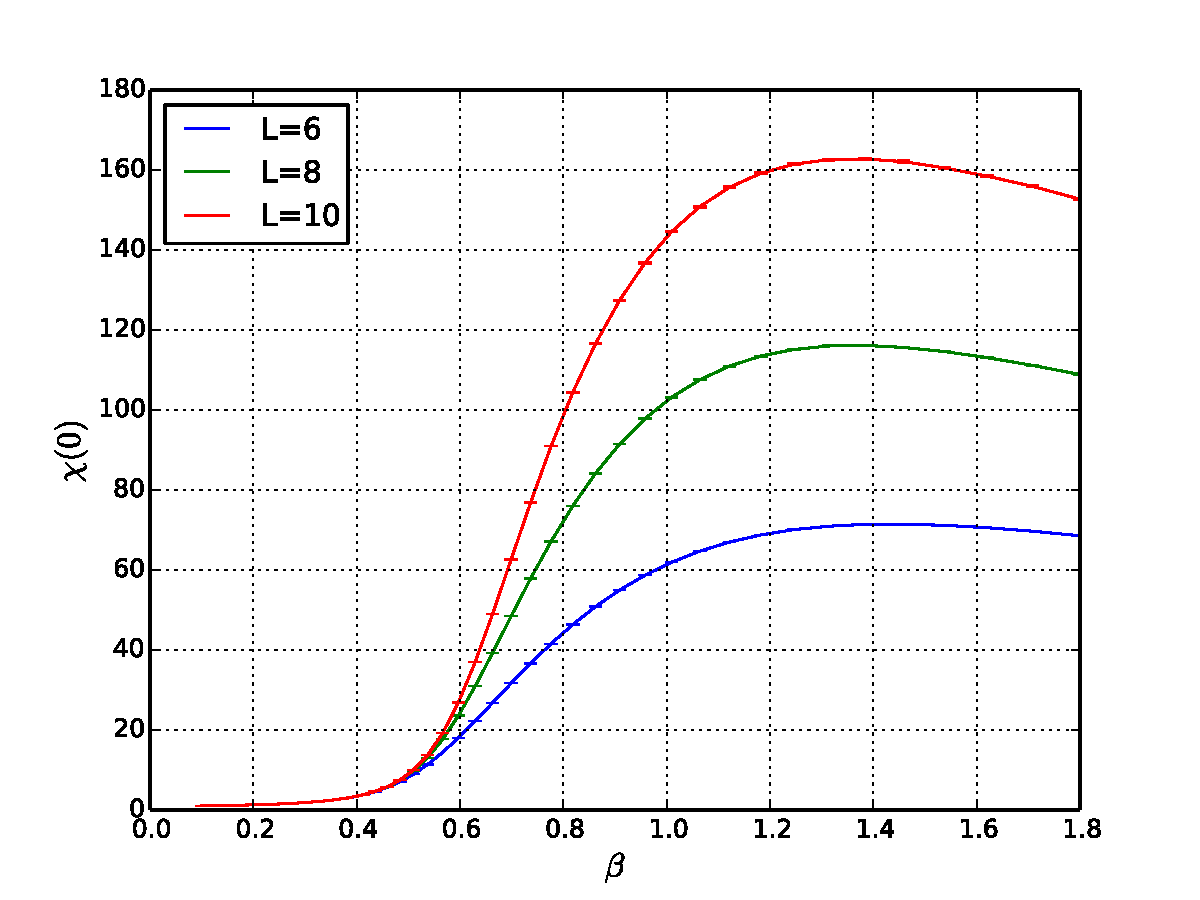
\includegraphics[width=0.6\textwidth]{img/chi.pdf}% 
  \caption{\label{fig:Chi} Spin glass susceptibility at zero momentum, $\chi(0)$, as a function of inverse temperature 
for system sizes $L=6,8,10$.}
\end{figure}


As the susceptibility does not show a behavior in accordance with the conventional 
finite size scaling theory for a second order transition, we move to study various 
cumulants and ratios of susceptibilities of the overlap parameter. We show the Binder ratio in Fig.~\ref{fig:Binder}. It does not display any signal of crossing. 
Indeed, the curves for different system sizes do not even tend to merge as the temperature 
is lowered.  Note that the Binder ratio corresponds to the fourth-order cumulant of the 
distribution, and 
%spin glass susceptibility at zero momentum. 
the possible issues related with the soft mode  
contributing to the zero momentum susceptibility should likely be canceled in the Binder ratio.

\begin{figure}[ht]
\centering

\centering
  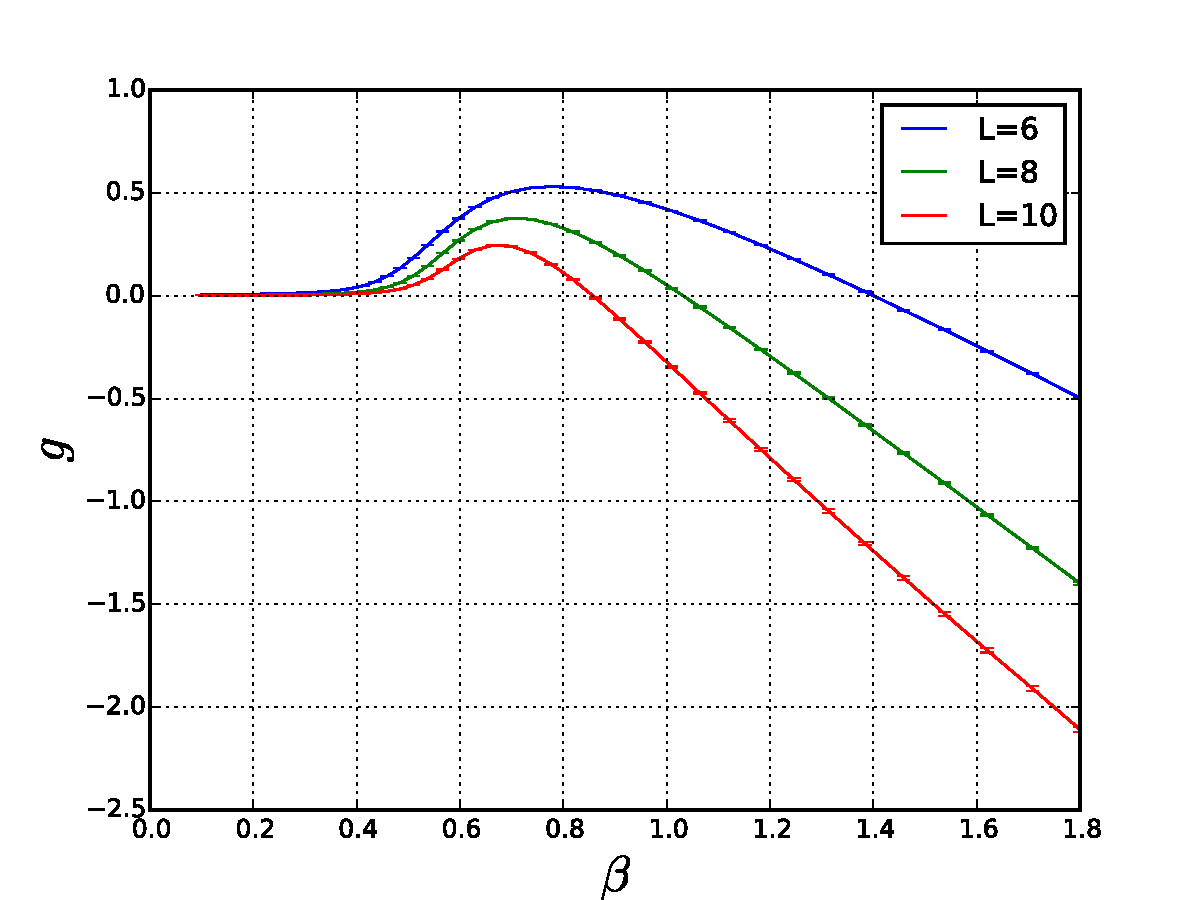
\includegraphics[width=0.6\textwidth]{img/binder.pdf}% Here is how to import EPS art
  \caption{\label{fig:b-h0} Binder ratio as a function of inverse temperature in the
range  $\beta=0.1\sim1.8$ for system sizes $L=6,8,10$.}
\label{fig:Binder}
\end{figure}

Fig.~\ref{fig:c-h0} displays the scaled correlation length. This is now a standard 
diagnosis for the detection of a spin glass transition. The correlation length is 
extracted from the Ornstein-Zernike form (Eq.~\ref{eq:corr}), and thus essentially given by the ratio 
between the zero and the smallest finite momentum susceptibilities. 
Similar to the Binder ratio, and consistent with other results in the literature, 
there is no crossing or even merging down to a rather low temperature~\cite{Young-Katzgraber2004}.

\begin{figure}[ht]
\centering

  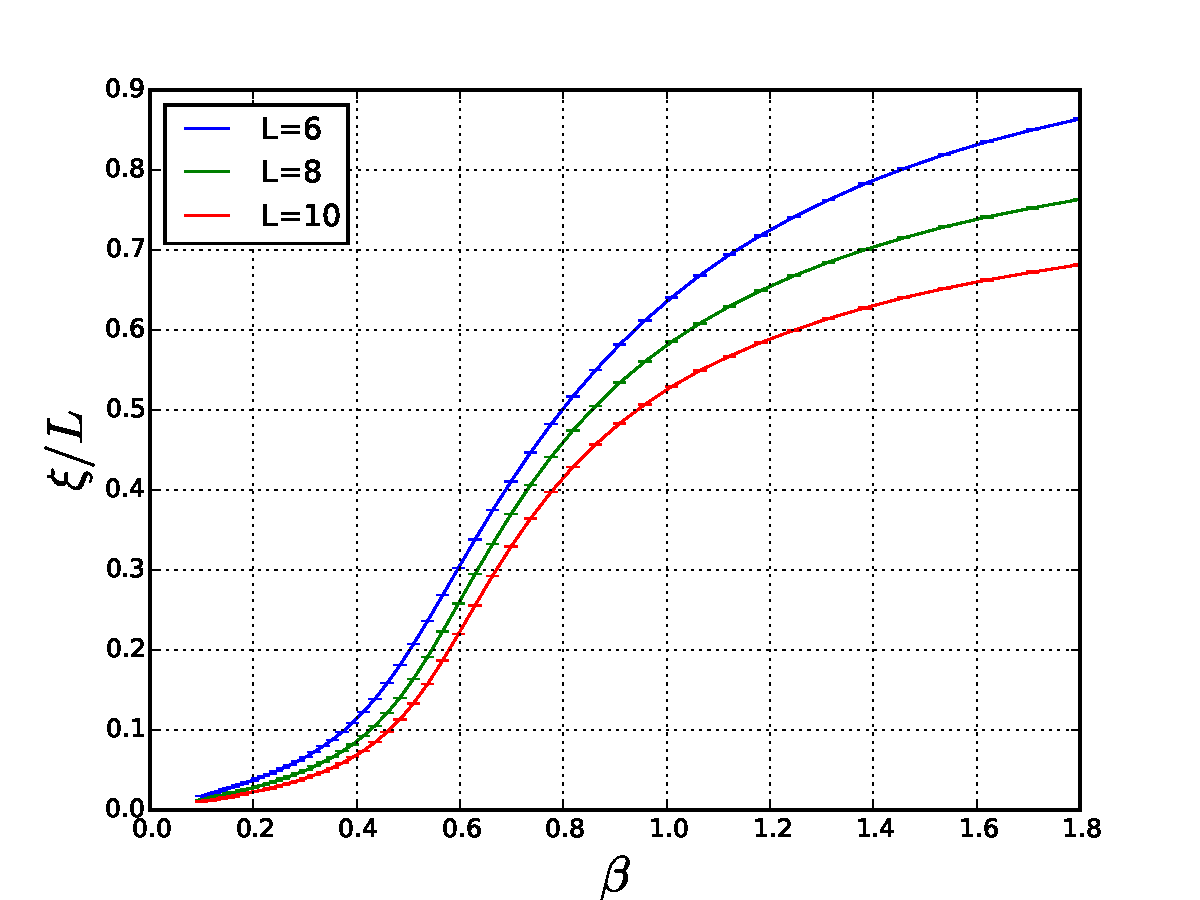
\includegraphics[width=0.6\textwidth]{img/corr.pdf}% Here is how to import EPS art
  \caption{\label{fig:c-h0} Scaled correlation length $\xi/L$ as a function of inverse temperature for system sizes $L=6,8,10$.  }
\end{figure}

From now on we focus on $R_{12}$. We performed simulations in zero field
where $R_{12}$ shows a crossing close to the expected critical temperature found from
the Binder ratio and the correlation. Therefore, the crossing in $R_{12}$ should 
be a viable indicator for the phase transition. Unfortunately, we find that $R_{12}$ is in 
general much noisier than other quantities. This is due to the fact that the sampling 
of higher momentum quantities is almost always characterized by larger statistical 
fluctuations. Taking the ratio between two susceptibilities at finite momenta clearly further
harms the quality of the data. To reduce the error bars we generate long runs and larger 
pools of disorder realizations (see Table \ref{tab:parameters}). This is the main reason we have generated a rather large number ($2.4 \times 10^5$) of realizations 
for the largest systems size we present here, and even more for smaller sizes. To further reduce the 
fluctuations, we impose all point group symmetries. For example, when we calculate 
$\chi(2\pi/L,0,0)$ we average the susceptibility at three different directions 
($\chi(2\pi/L,0,0)$, $\chi(0,2\pi/L,0)$, and $\chi(0,0,2\pi/L)$). This averaging implicitly assumes 
that the point group symmetry is restored which is justified only when the number of realizations
is rather large. 
 
\begin{figure}[ht]
\centering

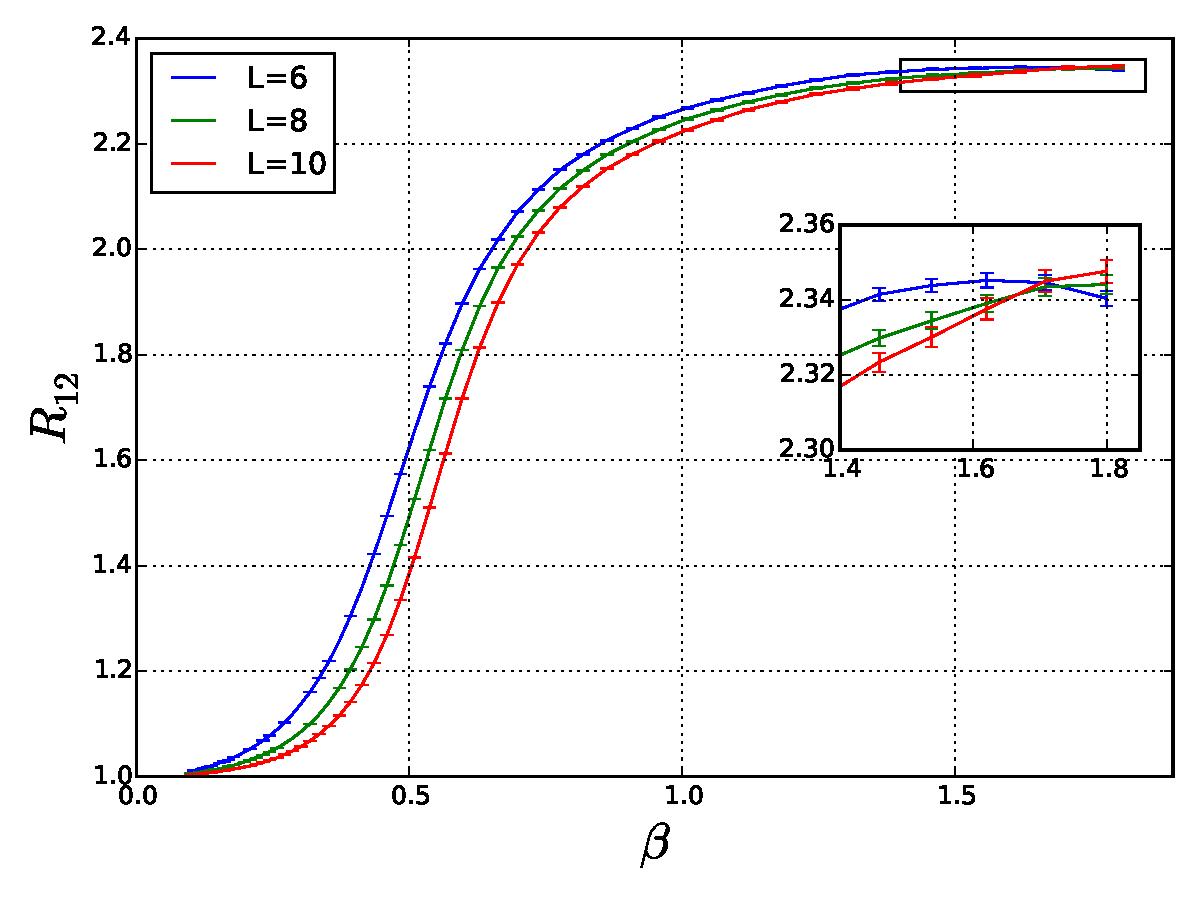
\includegraphics[width=0.6\textwidth]{img/r12.pdf}% Here is how to import EPS art
\caption{\label{fig:r12} $R_{12}$ as a function of inverse temperature for different system sizes. 
An intersection can be seen at around $T \approx 0.6$. We use the jackknife method to estimate 
the error bar from sample-to-sample variation.  
}
\end{figure}

Fig.~\ref{fig:r12} displays $R_{12}$. In contrast to other quantities, $R_{12}$ shows an intersection 
at about $T \approx 0.6$. We do not think we have sufficient data to perform a reasonably accurate finite size 
scaling analysis to report the exponent or even to quantify the correction \cite{Hasenbusch-etal-2008}.
Moreover, the data for $L=6$ does not seem to fit into a finite size scaling form with the curve bending downward.
Unfortunately, parallel tempering Monte Carlo is not robust enough for simulating larger lattices in a reasonable 
amount of time; this can be related to the temperature chaos \cite{Ritort-1994,Fernandez-etal-2013,Katzgraber-etal-2007}. The number of replicas needed to equilibrate the system also 
increases substantially as the system size increases, we already used $56$ temperature 
replicas for $L=10$ simulations. We plot $R_{12}$ versus the number of Monte 
Carlo sweeps in Fig.~\ref{fig:MCsteps}. We believe the data is sufficiently equilibrated for averaged quantities.
The major contribution to the error is from the limited number of disorder realizations. Fig.~\ref{fig:R12_l10_samples} shows $R_{12}$ 
for $L=10$ for different numbers of realizations. We clearly see that the data converges only when the number of realizations is fairly large.
This is one of the prominent hurdles of using higher momentum susceptibility as a diagnosis. 
We note that the effective one dimensional model also shows crossing behavior,
albeit the crossing points do not show a systematic trend\cite{Larson-etal-2013}.


\begin{figure}[ht]
\centering

  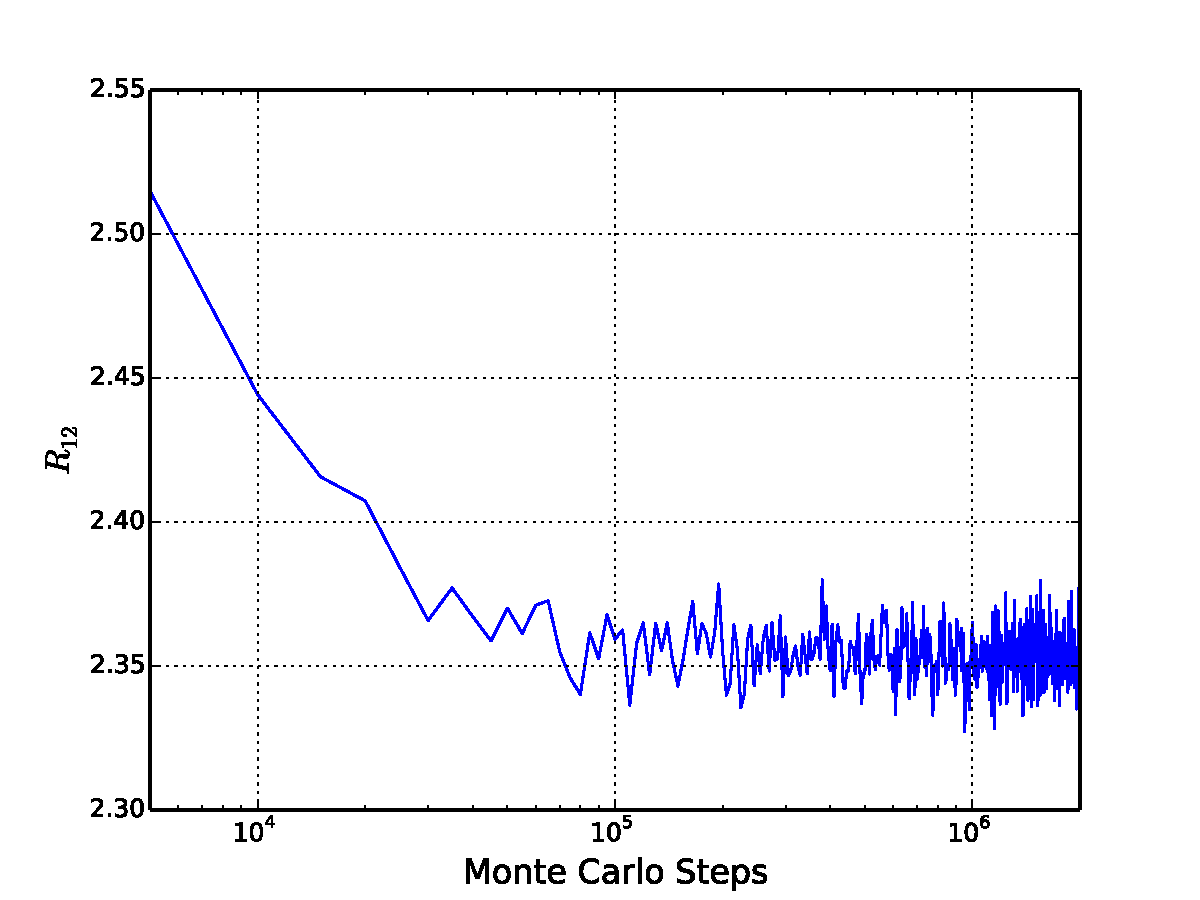
\includegraphics[width=0.6\textwidth]{img/eq_l10.pdf}
  \caption{\label{fig:MCsteps} $R_{12}$ for $L=10$ at $\beta=1.8$, as a function of the 
number of Monte Carlo sweeps.  We believe the averaged data is equilibrated 
for $10^6$  sweeps, and it passes the logarithm binning 
test \cite{Alvarez-etal-2010}. The main contribution to the error is from the realization 
averaging.}
\end{figure}


\begin{figure}[ht]
\centering
  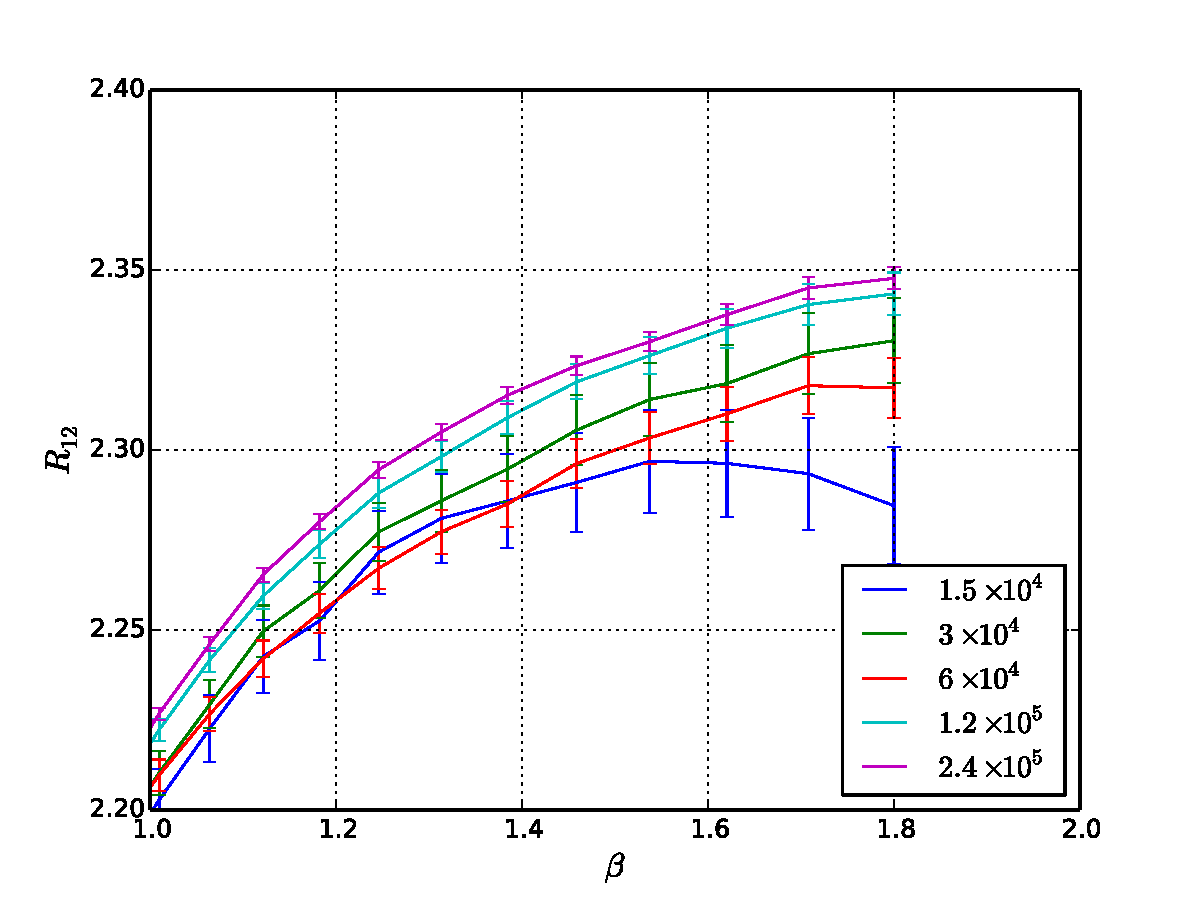
\includegraphics[width=0.6\textwidth]{img/R12_l10_samples.pdf}
  \caption{$R_{12}$ for $L=10$ and low temperatures ($\beta \geq 1.0$). We show five different numbers of 
realizations from fifteen thousand to two hundred forty thousand.}
\label{fig:R12_l10_samples}
\end{figure}


We studied the distribution of the susceptibilities. We calculated the susceptibility
for each disorder realization, and plotted the histogram at the lowest temperature,
$\beta=1.8$.
The distribution of susceptibilities are highly skewed. 
The mean of the distribution is dominated by rare
events, as suggested in Fig \ref{fig:hist_chi}. 
The non-Gaussian nature of the distribution suggests that the mean value might 
not be a good indicator. 


\begin{figure}[ht]
  \centering
  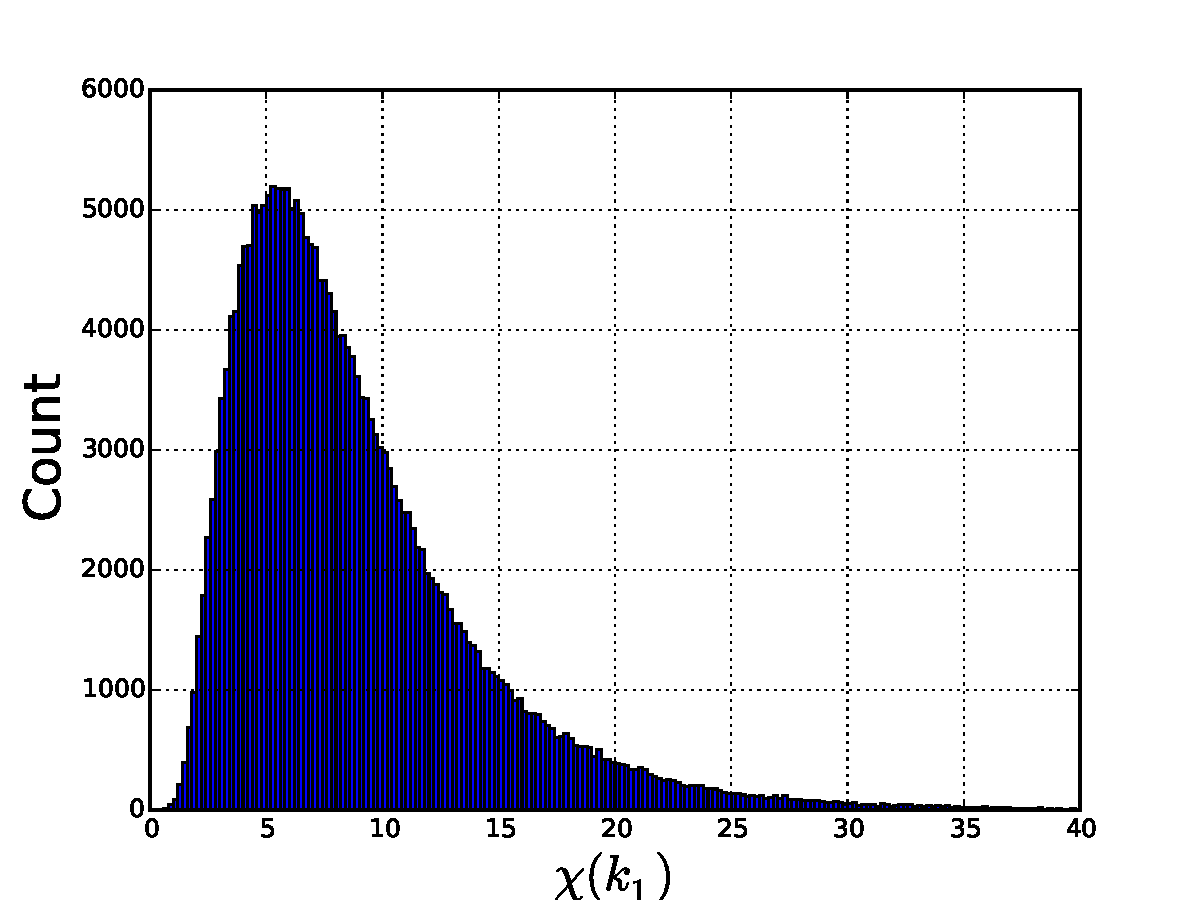
\includegraphics[width=0.7\textwidth]{img/chi_1_dist.pdf}
  \caption{Histogram for $\chi_1$ at low temperature.}
\label{fig:hist_chi}
\end{figure}

Here, we used the geometrical average \cite{PhysRevB.88.134204} over the susceptibilities to find $R_{12}$,
as shown in Fig \ref{fig:r12_gmean}.
We see that the lines are quite different from those obtained with arithmetic 
mean, and the crossings appear at different temperatures. 


\begin{figure}[ht]
  \centering
  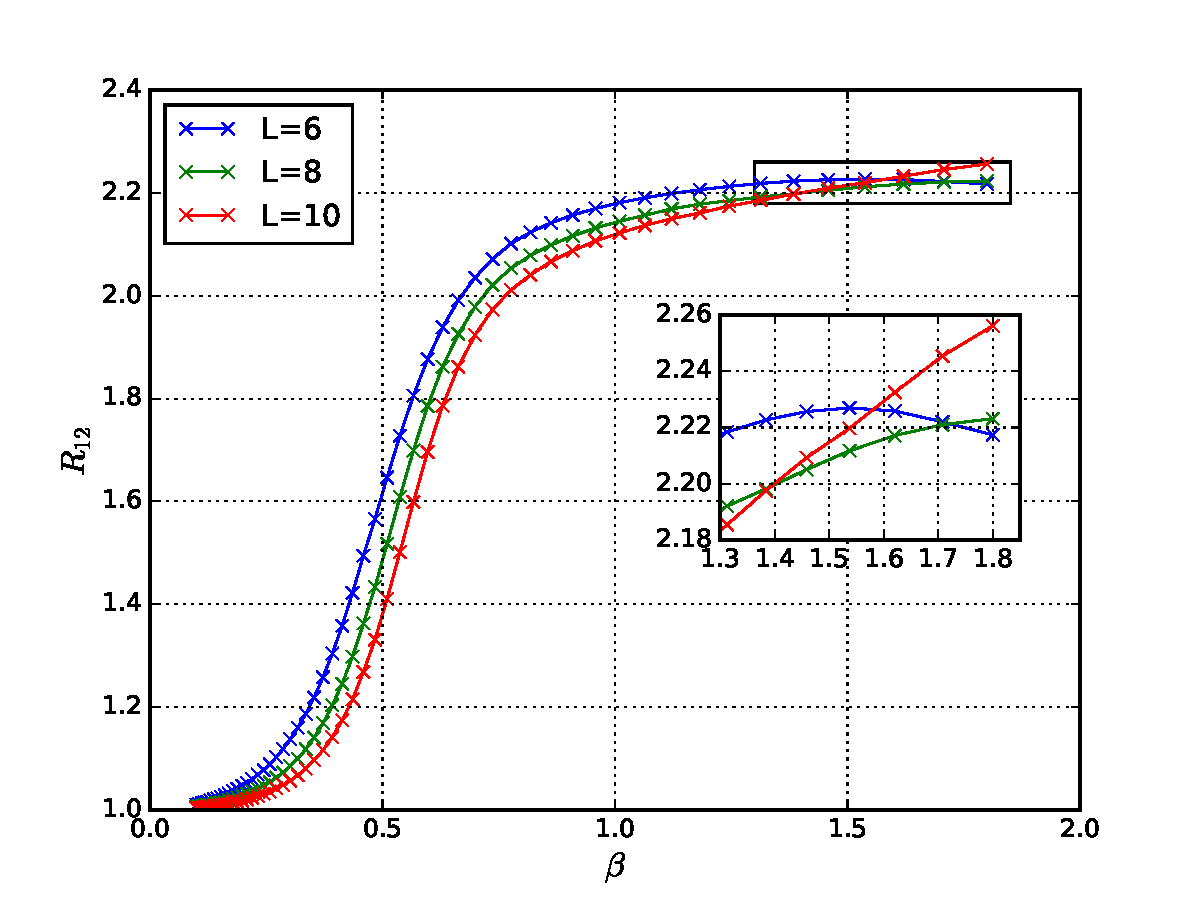
\includegraphics[width=0.7\textwidth]{img/r12_gmean_h01.pdf}
\caption{\label{fig:r12_gmean} $R_{12}$ calculated from the geometrical average
of susceptibilities, 
as a function of inverse temperature, for different system sizes. 
}
\end{figure}


\section{Discussions and Conclusions}
In summary, we perform Monte Carlo simulations of the three-dimensional
Edwards-Anderson model in a finite external field. The goal is to reexamine the 
long-standing problem of whether mean field behavior, specifically a spin glass phase, can
exist in such a model without time-reversal symmetry. We focus on the equilibrium quantities
of this notoriously difficult system. By taking advantage of the new commodity multi-threaded 
graphic computing units architecture we drastically reduce the computation time. The results 
for the Binder ratio and correlation length for different cluster sizes show no signal of an 
intersection, thus they point to the absence of a spin glass transition
as found in  previous studies. On the other hand, the ratio of susceptibilities 
$R_{12}$ does show an intersection for relatively small system sizes ($L=6,8,10$). 
We did perform simulations for larger system sizes, but this data 
is too noisy in particular for $R_{12}$ to draw a conclusion.
With the present system sizes and the statistical error bar, a rigorous data 
analysis does not seem to deliver unbiased information. 
This situation is rather discouraging, as simulations at this low temperature 
for much larger system sizes using the present method are daunting. 
Although we can not reach a definitive conclusion on whether a spin glass phase 
transition exists under a finite magnetic field,
we showed that the susceptibilities are not normally distributed and mean is 
dominated by rare events.
This motivated us to study the geometric average of the distribution. 
We showed that for different system sizes, there is similar crossing behavior 
in the $R_{12}$ calculated from the geometric average. 


The results are obtained with a very small external field, $h=0.1$. It is possible
that a larger field, such as $h=0.25$, would give us a stronger signal of crossing.
While this may give us a slightly clearer signal on the phase transition, should 
the transition exist at h=0.25, it would likely occur at a significantly lower temperature
which further jeopardizes the quality of the simulation data. As the result stands now, 
we cannot find a clear phase transition in h=0.1, and if there were no phase transition, 
it would also rule out the possibility of the transition occurring in a larger field. 
On the other hand, if we found evidence for the absence of a transition at h=0.25, we 
cannot determine if the spin glass phase would survive a smaller field like h=0.1. 
There is no simple rule of thumb which can be used to determine what value of h is 
the best for the purpose of answering the question on the existence of the transition 
under an external magnetic field. But we believe that the possible advantage of using  
a larger field does not outweigh the disadvantages, both in term of the difficultly
of the simulation, and its predictive power. 

 
Due to our efficient GPU implementation, we were able to leverage the computing
power of supercomputing clusters with GPU accelerators, and study a large number of disorder
realizations.
Our results show that with current numerical methods and computing capability obtainable 
results are still not robust enough to provide dispositive insight into the nature 
of a spin glass in 3D, and that we need either a different method to study the 
distribution of the data, or an exponential increase in computing power to gain 
more knowledge for this problem. 
We also think that any previous research based on the susceptibilities may 
suffer from the same problem, and the results from these work may be improved
by including a much larger of samples.

%This calls for a more thorough study on the model with different approaches.
%Possible directions include: 1) using models with continuous random distribution which are 
%easier to thermalize than that with bimodal distribution; 2) analyzing the
%data for the distribution of the overlap parameter, instead of average quantities. 

We notice a preprint before
we finished the present paper where the conditioning variate method
is used to expose the silent features from the data \cite{Baity-Jesi-etal-2014}. 


%\appendix

\section{System with L=16}

We further tested with a bigger system size, $L=16$. We used 11,200 realizations,
and divide them into four batches, each containing 2800 samples. We then calculated
the $R_{12}$ for the four batches, and compared them, as shown in Fig \ref{fig:l16_r12}. 
The results shows that a few thousand realizations is not enough, even for a 
system size of L=16. 


\begin{figure}[ht]
  \centering
  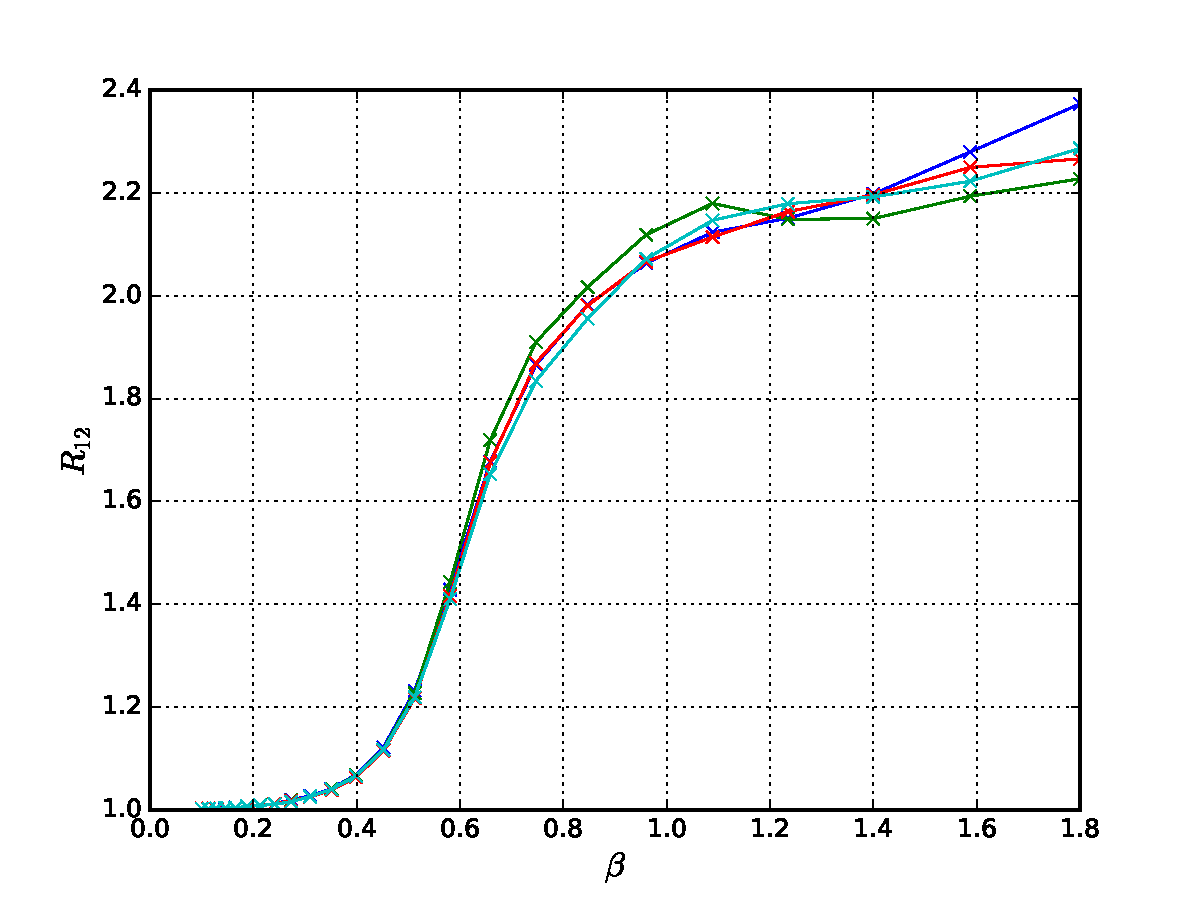
\includegraphics[width=0.7\textwidth]{img/l16_r12.pdf}
  \caption{$R_{12}$ for a larger system with $L=16$. We used four batches of samples,
each batch contains 2800 disorder realizations. The results shows that for
different batches $R_{12}$ is quite different, especially at low temperatures.
}
\label{fig:l16_r12}
\end{figure}


This work is sponsored by the NSF EPSCoR Cooperative Agreement No. EPS-1003897 with additional support 
from the Louisiana Board of Regents. This research were conducted with high 
performance computational resources provided by 
Louisiana State University (http://www.hpc.lsu.edu). We thank Helmut Katzgraber and Karen 
Tomko for useful conversations. We thank the following collaborators: Bhupender Thakur, Ariane Papke, Sean Hall, and Cade Thomasson. 


%%% Local Variables:
%%% mode: latex
%%% TeX-master: "../thesis"
%%% End:
